% Appendix E figure of "Galashin's Conjecture 4.3 via a convex gradient": Lemma 5 (the component reduction) on actual cells.
% Source in the paper's own fonts at the text width (6.5in). It adds no assertion and is used in no proof.
% Every value drawn is read from Lean output lines (SHA-256 of the lines), evaluated by the formal definitions of
% Conj43.Reduction (component, labelsOf, restrictEntry; the restricted angles; the gaps):
%   picture D156 2ecff4bddbba473d10809ee2af4596fa892aea4f6f63712cc77e90ff8c5bf3e8
%   picture D157 d7abf0f49dfca6a333a41639fd6dd5e9be6b8db6157da698a54178d6a58908fb
%   picture D158 12b716cdfb0304f9704344acc3b02e2295c4cbe05c38373c39b2357a42c79e0e
%   picture D159 8b8f96a4443316b314e7b4f41142ec8e5fd10c6a072364ccb9fc283494ee08fd
% Build: pdflatex <this file> && pdftocairo -svg <this file>.pdf <this file>.svg
\documentclass[11pt]{standalone}
\usepackage[T1]{fontenc}
\usepackage{lmodern}
\usepackage{amsmath,amssymb}
\usepackage{tikz}
\definecolor{ink}{HTML}{233740}
\definecolor{muted}{HTML}{65757D}
\definecolor{pblue}{HTML}{0072B2}
\definecolor{qochre}{HTML}{B87827}
\definecolor{addg}{HTML}{009E73}
\definecolor{remv}{HTML}{D55E00}
\begin{document}
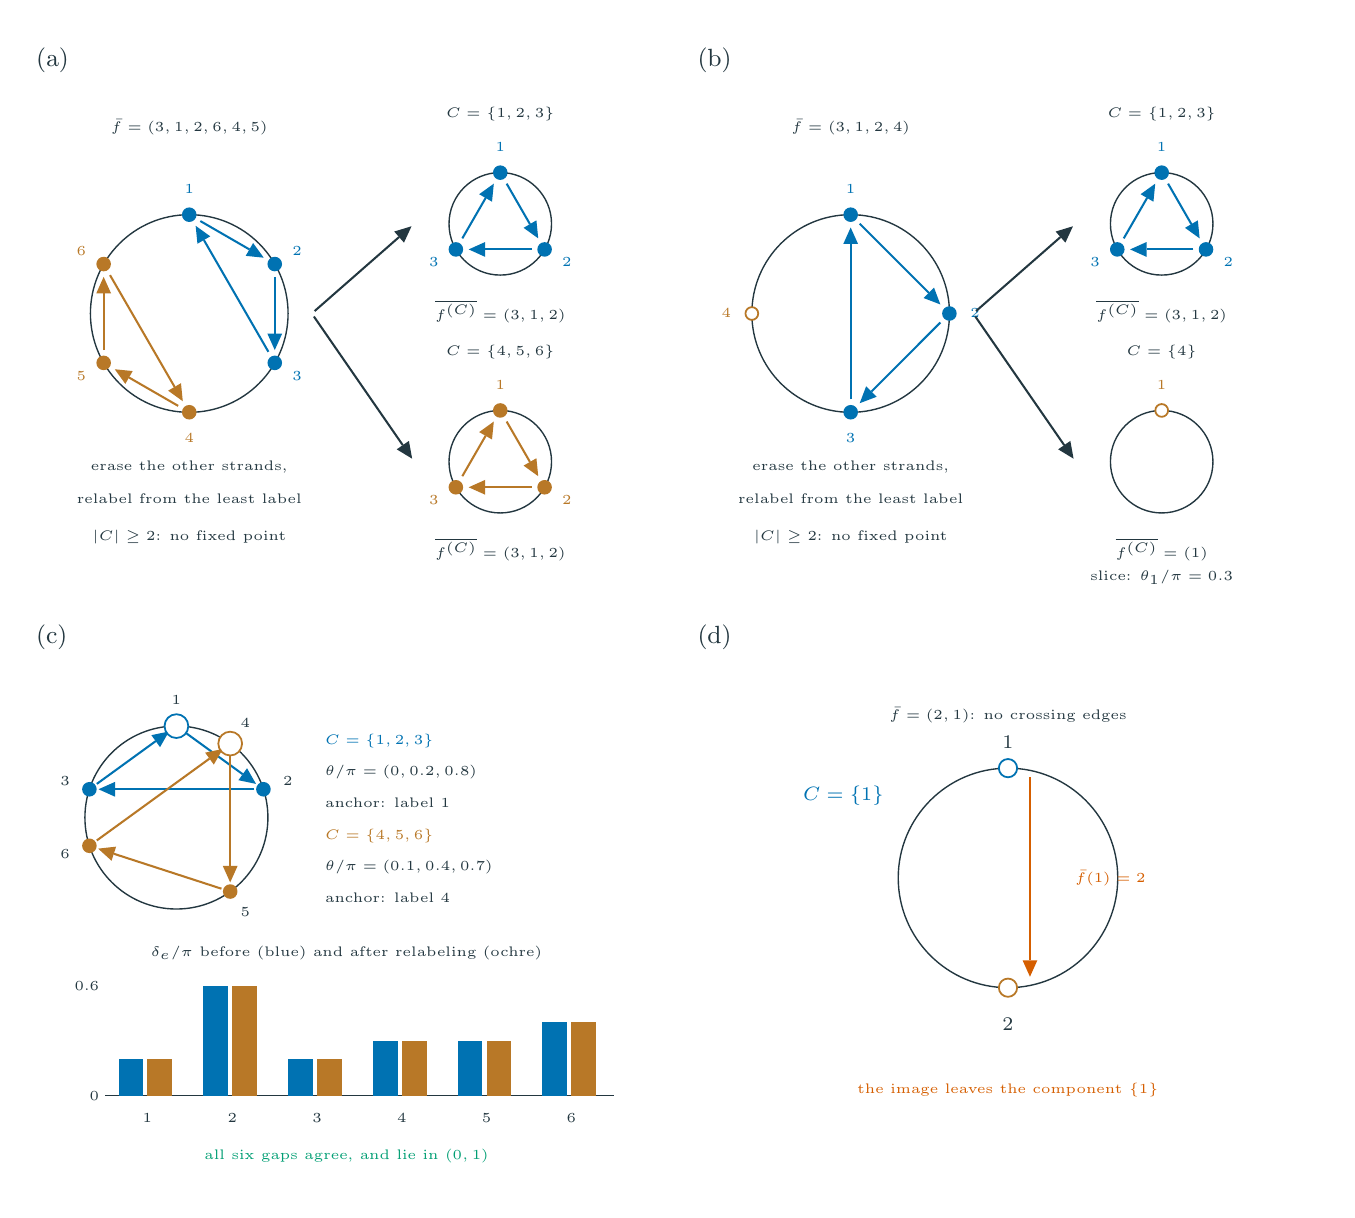
\begin{tikzpicture}[x=1cm,y=1cm]
\useasboundingbox (-0.1,-14.462) rectangle (16.4,0.3);
\node[anchor=north west, inner sep=0pt, font=\small, text=ink] at (0.000,0.050) {(a)};
\node[anchor=center, inner sep=0pt, text=ink, font=\tiny] at (1.952,-0.960) {$\bar f=(3,1,2,6,4,5)$};
\path[fill=white, draw=ink, line width=0.50pt] (1.952,-3.330) circle (1.255);
\draw[pblue, line width=0.74pt] (2.093,-2.156) -- (2.716,-2.516);
\fill[pblue] (2.898,-2.621) -- (2.669,-2.598) -- (2.763,-2.435) -- cycle;
\draw[pblue, line width=0.74pt] (3.038,-2.865) -- (3.038,-3.585);
\fill[pblue] (3.038,-3.794) -- (2.944,-3.585) -- (3.132,-3.585) -- cycle;
\draw[pblue, line width=0.74pt] (2.957,-3.816) -- (2.138,-2.397);
\fill[pblue] (2.033,-2.216) -- (2.219,-2.350) -- (2.056,-2.444) -- cycle;
\draw[qochre, line width=0.74pt] (1.811,-4.503) -- (1.187,-4.143);
\fill[qochre] (1.006,-4.038) -- (1.234,-4.061) -- (1.140,-4.224) -- cycle;
\draw[qochre, line width=0.74pt] (0.865,-3.794) -- (0.865,-3.074);
\fill[qochre] (0.865,-2.865) -- (0.959,-3.074) -- (0.771,-3.074) -- cycle;
\draw[qochre, line width=0.74pt] (0.946,-2.843) -- (1.766,-4.262);
\fill[qochre] (1.870,-4.444) -- (1.684,-4.310) -- (1.847,-4.215) -- cycle;
\path[fill=pblue, draw=pblue, line width=0.64pt] (1.952,-2.075) circle (0.081);
\node[anchor=center, inner sep=0pt, text=pblue, font=\tiny] at (1.952,-1.750) {1};
\path[fill=pblue, draw=pblue, line width=0.64pt] (3.038,-2.702) circle (0.081);
\node[anchor=center, inner sep=0pt, text=pblue, font=\tiny] at (3.320,-2.540) {2};
\path[fill=pblue, draw=pblue, line width=0.64pt] (3.038,-3.957) circle (0.081);
\node[anchor=center, inner sep=0pt, text=pblue, font=\tiny] at (3.320,-4.120) {3};
\path[fill=qochre, draw=qochre, line width=0.64pt] (1.952,-4.584) circle (0.081);
\node[anchor=center, inner sep=0pt, text=qochre, font=\tiny] at (1.952,-4.910) {4};
\path[fill=qochre, draw=qochre, line width=0.64pt] (0.865,-3.957) circle (0.081);
\node[anchor=center, inner sep=0pt, text=qochre, font=\tiny] at (0.583,-4.120) {5};
\path[fill=qochre, draw=qochre, line width=0.64pt] (0.865,-2.702) circle (0.081);
\node[anchor=center, inner sep=0pt, text=qochre, font=\tiny] at (0.583,-2.540) {6};
\path[fill=white, draw=ink, line width=0.50pt] (5.902,-2.191) circle (0.651);
\draw[pblue, line width=0.74pt] (5.983,-1.681) -- (6.279,-2.195);
\fill[pblue] (6.384,-2.376) -- (6.198,-2.242) -- (6.361,-2.147) -- cycle;
\draw[pblue, line width=0.74pt] (6.303,-2.516) -- (5.710,-2.516);
\fill[pblue] (5.501,-2.516) -- (5.710,-2.422) -- (5.710,-2.611) -- cycle;
\draw[pblue, line width=0.74pt] (5.420,-2.376) -- (5.716,-1.863);
\fill[pblue] (5.820,-1.681) -- (5.797,-1.910) -- (5.634,-1.815) -- cycle;
\path[fill=pblue, draw=pblue, line width=0.64pt] (5.902,-1.541) circle (0.081);
\node[anchor=center, inner sep=0pt, text=pblue, font=\tiny] at (5.902,-1.215) {1};
\path[fill=pblue, draw=pblue, line width=0.64pt] (6.465,-2.516) circle (0.081);
\node[anchor=center, inner sep=0pt, text=pblue, font=\tiny] at (6.747,-2.679) {2};
\path[fill=pblue, draw=pblue, line width=0.64pt] (5.338,-2.516) circle (0.081);
\node[anchor=center, inner sep=0pt, text=pblue, font=\tiny] at (5.057,-2.679) {3};
\node[anchor=center, inner sep=0pt, text=ink, font=\tiny] at (5.902,-0.797) {$C=\{1,2,3\}$};
\node[anchor=center, inner sep=0pt, text=ink, font=\tiny] at (5.902,-3.306) {$\overline{f^{(C)}}=(3,1,2)$};
\draw[ink, line width=0.74pt] (3.544,-3.299) -- (4.617,-2.359);
\fill[ink] (4.775,-2.222) -- (4.679,-2.430) -- (4.555,-2.289) -- cycle;
\path[fill=white, draw=ink, line width=0.50pt] (5.902,-5.212) circle (0.651);
\draw[qochre, line width=0.74pt] (5.983,-4.702) -- (6.279,-5.215);
\fill[qochre] (6.384,-5.396) -- (6.198,-5.262) -- (6.361,-5.168) -- cycle;
\draw[qochre, line width=0.74pt] (6.303,-5.537) -- (5.710,-5.537);
\fill[qochre] (5.501,-5.537) -- (5.710,-5.443) -- (5.710,-5.631) -- cycle;
\draw[qochre, line width=0.74pt] (5.420,-5.396) -- (5.716,-4.883);
\fill[qochre] (5.820,-4.702) -- (5.797,-4.930) -- (5.634,-4.836) -- cycle;
\path[fill=qochre, draw=qochre, line width=0.64pt] (5.902,-4.561) circle (0.081);
\node[anchor=center, inner sep=0pt, text=qochre, font=\tiny] at (5.902,-4.236) {1};
\path[fill=qochre, draw=qochre, line width=0.64pt] (6.465,-5.537) circle (0.081);
\node[anchor=center, inner sep=0pt, text=qochre, font=\tiny] at (6.747,-5.700) {2};
\path[fill=qochre, draw=qochre, line width=0.64pt] (5.338,-5.537) circle (0.081);
\node[anchor=center, inner sep=0pt, text=qochre, font=\tiny] at (5.057,-5.700) {3};
\node[anchor=center, inner sep=0pt, text=ink, font=\tiny] at (5.902,-3.818) {$C=\{4,5,6\}$};
\node[anchor=center, inner sep=0pt, text=ink, font=\tiny] at (5.902,-6.327) {$\overline{f^{(C)}}=(3,1,2)$};
\draw[ink, line width=0.74pt] (3.535,-3.368) -- (4.664,-5.002);
\fill[ink] (4.783,-5.174) -- (4.587,-5.055) -- (4.742,-4.948) -- cycle;
\node[anchor=center, inner sep=0pt, text=ink, font=\tiny] at (1.952,-5.281) {erase the other strands,};
\node[anchor=center, inner sep=0pt, text=ink, font=\tiny] at (1.952,-5.676) {relabel from the least label};
\node[anchor=center, inner sep=0pt, text=ink, font=\tiny] at (1.952,-6.164) {$|C|\ge2$: no fixed point};
\node[anchor=north west, inner sep=0pt, font=\small, text=ink] at (8.400,0.050) {(b)};
\node[anchor=center, inner sep=0pt, text=ink, font=\tiny] at (10.352,-0.960) {$\bar f=(3,1,2,4)$};
\path[fill=white, draw=ink, line width=0.50pt] (10.352,-3.330) circle (1.255);
\draw[pblue, line width=0.74pt] (10.467,-2.190) -- (11.344,-3.067);
\fill[pblue] (11.491,-3.215) -- (11.277,-3.133) -- (11.410,-3.000) -- cycle;
\draw[pblue, line width=0.74pt] (11.491,-3.445) -- (10.615,-4.322);
\fill[pblue] (10.467,-4.469) -- (10.548,-4.255) -- (10.681,-4.388) -- cycle;
\draw[pblue, line width=0.74pt] (10.352,-4.422) -- (10.352,-2.447);
\fill[pblue] (10.352,-2.238) -- (10.446,-2.447) -- (10.258,-2.447) -- cycle;
\path[fill=pblue, draw=pblue, line width=0.64pt] (10.352,-2.075) circle (0.081);
\node[anchor=center, inner sep=0pt, text=pblue, font=\tiny] at (10.352,-1.750) {1};
\path[fill=pblue, draw=pblue, line width=0.64pt] (11.606,-3.330) circle (0.081);
\node[anchor=center, inner sep=0pt, text=pblue, font=\tiny] at (11.932,-3.330) {2};
\path[fill=pblue, draw=pblue, line width=0.64pt] (10.352,-4.584) circle (0.081);
\node[anchor=center, inner sep=0pt, text=pblue, font=\tiny] at (10.352,-4.910) {3};
\path[fill=white, draw=qochre, line width=0.64pt] (9.097,-3.330) circle (0.081);
\node[anchor=center, inner sep=0pt, text=qochre, font=\tiny] at (8.772,-3.330) {4};
\path[fill=white, draw=ink, line width=0.50pt] (14.302,-2.191) circle (0.651);
\draw[pblue, line width=0.74pt] (14.383,-1.681) -- (14.679,-2.195);
\fill[pblue] (14.784,-2.376) -- (14.598,-2.242) -- (14.761,-2.147) -- cycle;
\draw[pblue, line width=0.74pt] (14.703,-2.516) -- (14.110,-2.516);
\fill[pblue] (13.901,-2.516) -- (14.110,-2.422) -- (14.110,-2.611) -- cycle;
\draw[pblue, line width=0.74pt] (13.820,-2.376) -- (14.116,-1.863);
\fill[pblue] (14.220,-1.681) -- (14.197,-1.910) -- (14.034,-1.815) -- cycle;
\path[fill=pblue, draw=pblue, line width=0.64pt] (14.302,-1.541) circle (0.081);
\node[anchor=center, inner sep=0pt, text=pblue, font=\tiny] at (14.302,-1.215) {1};
\path[fill=pblue, draw=pblue, line width=0.64pt] (14.865,-2.516) circle (0.081);
\node[anchor=center, inner sep=0pt, text=pblue, font=\tiny] at (15.147,-2.679) {2};
\path[fill=pblue, draw=pblue, line width=0.64pt] (13.738,-2.516) circle (0.081);
\node[anchor=center, inner sep=0pt, text=pblue, font=\tiny] at (13.457,-2.679) {3};
\node[anchor=center, inner sep=0pt, text=ink, font=\tiny] at (14.302,-0.797) {$C=\{1,2,3\}$};
\node[anchor=center, inner sep=0pt, text=ink, font=\tiny] at (14.302,-3.306) {$\overline{f^{(C)}}=(3,1,2)$};
\draw[ink, line width=0.74pt] (11.944,-3.299) -- (13.017,-2.359);
\fill[ink] (13.175,-2.222) -- (13.079,-2.430) -- (12.955,-2.289) -- cycle;
\path[fill=white, draw=ink, line width=0.50pt] (14.302,-5.212) circle (0.651);
\path[fill=white, draw=qochre, line width=0.64pt] (14.302,-4.561) circle (0.081);
\node[anchor=center, inner sep=0pt, text=qochre, font=\tiny] at (14.302,-4.236) {1};
\node[anchor=center, inner sep=0pt, text=ink, font=\tiny] at (14.302,-3.818) {$C=\{4\}$};
\node[anchor=center, inner sep=0pt, text=ink, font=\tiny] at (14.302,-6.327) {$\overline{f^{(C)}}=(1)$};
\node[anchor=center, inner sep=0pt, text=ink, font=\tiny] at (14.302,-6.676) {slice: $\theta_1/\pi=0.3$};
\draw[ink, line width=0.74pt] (11.935,-3.368) -- (13.064,-5.002);
\fill[ink] (13.183,-5.174) -- (12.987,-5.055) -- (13.142,-4.948) -- cycle;
\node[anchor=center, inner sep=0pt, text=ink, font=\tiny] at (10.352,-5.281) {erase the other strands,};
\node[anchor=center, inner sep=0pt, text=ink, font=\tiny] at (10.352,-5.676) {relabel from the least label};
\node[anchor=center, inner sep=0pt, text=ink, font=\tiny] at (10.352,-6.164) {$|C|\ge2$: no fixed point};
\node[anchor=north west, inner sep=0pt, font=\small, text=ink] at (0.000,-7.281) {(c)};
\path[fill=white, draw=ink, line width=0.50pt] (1.789,-9.731) circle (1.162);
\draw[pblue, line width=0.74pt] (1.883,-8.638) -- (2.631,-9.181);
\fill[pblue] (2.800,-9.304) -- (2.576,-9.257) -- (2.686,-9.105) -- cycle;
\draw[pblue, line width=0.74pt] (2.778,-9.372) -- (1.010,-9.372);
\fill[pblue] (0.800,-9.372) -- (1.010,-9.278) -- (1.010,-9.467) -- cycle;
\draw[pblue, line width=0.74pt] (0.778,-9.304) -- (1.526,-8.761);
\fill[pblue] (1.695,-8.638) -- (1.581,-8.837) -- (1.471,-8.685) -- cycle;
\draw[qochre, line width=0.74pt] (2.472,-8.908) -- (2.472,-10.346);
\fill[qochre] (2.472,-10.555) -- (2.378,-10.346) -- (2.566,-10.346) -- cycle;
\draw[qochre, line width=0.74pt] (2.361,-10.635) -- (0.994,-10.191);
\fill[qochre] (0.795,-10.126) -- (1.023,-10.101) -- (0.965,-10.280) -- cycle;
\draw[qochre, line width=0.74pt] (0.778,-10.022) -- (2.209,-8.983);
\fill[qochre] (2.378,-8.860) -- (2.264,-9.059) -- (2.154,-8.907) -- cycle;
\path[fill=pblue, draw=pblue, line width=0.64pt] (1.789,-8.570) circle (0.081);
\node[anchor=center, inner sep=0pt, text=ink, font=\tiny] at (1.789,-8.244) {1};
\path[fill=white, draw=pblue, line width=0.64pt] (1.789,-8.570) circle (0.151);
\path[fill=pblue, draw=pblue, line width=0.64pt] (2.894,-9.372) circle (0.081);
\node[anchor=center, inner sep=0pt, text=ink, font=\tiny] at (3.203,-9.272) {2};
\path[fill=pblue, draw=pblue, line width=0.64pt] (0.684,-9.372) circle (0.081);
\node[anchor=center, inner sep=0pt, text=ink, font=\tiny] at (0.375,-9.272) {3};
\path[fill=qochre, draw=qochre, line width=0.64pt] (2.472,-8.792) circle (0.081);
\node[anchor=center, inner sep=0pt, text=ink, font=\tiny] at (2.663,-8.528) {4};
\path[fill=white, draw=qochre, line width=0.64pt] (2.472,-8.792) circle (0.151);
\path[fill=qochre, draw=qochre, line width=0.64pt] (2.472,-10.671) circle (0.081);
\node[anchor=center, inner sep=0pt, text=ink, font=\tiny] at (2.663,-10.935) {5};
\path[fill=qochre, draw=qochre, line width=0.64pt] (0.684,-10.090) circle (0.081);
\node[anchor=center, inner sep=0pt, text=ink, font=\tiny] at (0.375,-10.191) {6};
\node[anchor=west, inner sep=0pt, text=pblue, font=\tiny] at (3.671,-8.756) {$C=\{1,2,3\}$};
\node[anchor=west, inner sep=0pt, text=ink, font=\tiny] at (3.671,-9.151) {$\theta/\pi=(0,0.2,0.8)$};
\node[anchor=west, inner sep=0pt, text=ink, font=\tiny] at (3.671,-9.546) {anchor: label 1};
\node[anchor=west, inner sep=0pt, text=qochre, font=\tiny] at (3.671,-9.964) {$C=\{4,5,6\}$};
\node[anchor=west, inner sep=0pt, text=ink, font=\tiny] at (3.671,-10.359) {$\theta/\pi=(0.1,0.4,0.7)$};
\node[anchor=west, inner sep=0pt, text=ink, font=\tiny] at (3.671,-10.754) {anchor: label 4};
\node[anchor=center, inner sep=0pt, text=ink, font=\tiny] at (3.950,-11.451) {$\delta_e/\pi$ before (blue) and after relabeling (ochre)};
\draw[ink, line width=0.40pt] (0.883,-13.263) -- (7.342,-13.263);
\node[anchor=east, inner sep=0pt, text=ink, font=\tiny] at (0.813,-11.869) {0.6};
\node[anchor=east, inner sep=0pt, text=ink, font=\tiny] at (0.813,-13.263) {0};
\fill[pblue] (1.055,-12.799) rectangle (1.370,-13.263);
\fill[pblue] (2.132,-11.869) rectangle (2.447,-13.263);
\fill[pblue] (3.208,-12.799) rectangle (3.523,-13.263);
\fill[pblue] (4.285,-12.566) rectangle (4.600,-13.263);
\fill[pblue] (5.362,-12.566) rectangle (5.676,-13.263);
\fill[pblue] (6.438,-12.334) rectangle (6.753,-13.263);
\fill[qochre] (1.421,-12.799) rectangle (1.736,-13.263);
\fill[qochre] (2.498,-11.869) rectangle (2.813,-13.263);
\fill[qochre] (3.574,-12.799) rectangle (3.889,-13.263);
\fill[qochre] (4.651,-12.566) rectangle (4.966,-13.263);
\fill[qochre] (5.728,-12.566) rectangle (6.042,-13.263);
\fill[qochre] (6.804,-12.334) rectangle (7.119,-13.263);
\node[anchor=center, inner sep=0pt, text=ink, font=\tiny] at (1.421,-13.542) {1};
\node[anchor=center, inner sep=0pt, text=ink, font=\tiny] at (2.498,-13.542) {2};
\node[anchor=center, inner sep=0pt, text=ink, font=\tiny] at (3.574,-13.542) {3};
\node[anchor=center, inner sep=0pt, text=ink, font=\tiny] at (4.651,-13.542) {4};
\node[anchor=center, inner sep=0pt, text=ink, font=\tiny] at (5.728,-13.542) {5};
\node[anchor=center, inner sep=0pt, text=ink, font=\tiny] at (6.804,-13.542) {6};
\node[anchor=center, inner sep=0pt, text=addg, font=\tiny] at (3.950,-14.030) {all six gaps agree, and lie in $(0,1)$};
\node[anchor=north west, inner sep=0pt, font=\small, text=ink] at (8.400,-7.281) {(d)};
\node[anchor=center, inner sep=0pt, text=ink, font=\tiny] at (12.350,-8.430) {$\bar f=(2,1)$: no crossing edges};
\path[fill=white, draw=ink, line width=0.50pt] (12.350,-10.498) circle (1.394);
\path[fill=white, draw=pblue, line width=0.64pt] (12.350,-9.104) circle (0.116);
\path[fill=white, draw=qochre, line width=0.64pt] (12.350,-11.892) circle (0.116);
\node[anchor=center, inner sep=0pt, text=ink, font=\scriptsize] at (12.350,-8.779) {1};
\node[anchor=center, inner sep=0pt, text=ink, font=\scriptsize] at (12.350,-12.357) {2};
\draw[remv, line width=0.74pt] (12.629,-9.220) -- (12.629,-11.544);
\fill[remv] (12.629,-11.753) -- (12.535,-11.544) -- (12.723,-11.544) -- cycle;
\node[anchor=center, inner sep=0pt, text=remv, font=\tiny] at (13.651,-10.498) {$\bar f(1)=2$};
\node[anchor=center, inner sep=0pt, text=pblue, font=\scriptsize] at (10.259,-9.453) {$C=\{1\}$};
\node[anchor=center, inner sep=0pt, text=remv, font=\tiny] at (12.350,-13.194) {the image leaves the component $\{1\}$};
\end{tikzpicture}
\end{document}
